%%
%% This is file `sample-sigconf.tex',
%% generated with the docstrip utility.
%%
%% The original source files were:
%%
%% samples.dtx  (with options: `sigconf')
%% 
%% IMPORTANT NOTICE:
%% 
%% For the copyright see the source file.
%% 
%% Any modified versions of this file must be renamed
%% with new filenames distinct from sample-sigconf.tex.
%% 
%% For distribution of the original source see the terms
%% for copying and modification in the file samples.dtx.
%% 
%% This generated file may be distributed as long as the
%% original source files, as listed above, are part of the
%% same distribution. (The sources need not necessarily be
%% in the same archive or directory.)
%%
%% The first command in your LaTeX source must be the \documentclass command.
\documentclass[sigconf, review]{acmart}




%%
%% \BibTeX command to typeset BibTeX logo in the docs
\AtBeginDocument{%
	\providecommand\BibTeX{{%
			\normalfont B\kern-0.5em{\scshape i\kern-0.25em b}\kern-0.8em\TeX}}}

%% Rights management information.  This information is sent to you
%% when you complete the rights form.  These commands have SAMPLE
%% values in them; it is your responsibility as an author to replace
%% the commands and values with those provided to you when you
%% complete the rights form.
\setcopyright{acmcopyright}
\copyrightyear{2020}
\acmYear{2020}
\acmDOI{10.1145/1122445.1122456}

%% These commands are for a PROCEEDINGS abstract or paper.
\acmConference[MSR '20]{MSR '20: Mining Software Repositories}{May 25--26, 2020}{Yongsan-gu, Seoul, South Korea}
\acmBooktitle{MSR '20: Mining Software Repositories,
	May 25--26, 2020, Yongsan-gu, Seoul, South Korea}
\acmPrice{15.00}
\acmISBN{978-1-4503-9999-9/18/06}


%%
%% Submission ID.
%% Use this when submitting an article to a sponsored event. You'll
%% receive a unique submission ID from the organizers
%% of the event, and this ID should be used as the parameter to this command.
%%\acmSubmissionID{123-A56-BU3}

%%
%% The majority of ACM publications use numbered citations and
%% references.  The command \citestyle{authoryear} switches to the
%% "author year" style.
%%
%% If you are preparing content for an event
%% sponsored by ACM SIGGRAPH, you must use the "author year" style of
%% citations and references.
%% Uncommenting
%% the next command will enable that style.
%%\citestyle{acmauthoryear}





\usepackage{listings}
\usepackage{color}

\definecolor{dkgreen}{rgb}{0,0.6,0}
\definecolor{gray}{rgb}{0.5,0.5,0.5}
\definecolor{mauve}{rgb}{0.58,0,0.82}

\lstset{frame=tb,
	language=Python,
	aboveskip=3mm,
	belowskip=3mm,
	showstringspaces=false,
	columns=flexible,
	basicstyle={\small\ttfamily},
	numbers=none,
	numberstyle=\tiny\color{gray},
	keywordstyle=\color{blue},
	commentstyle=\color{dkgreen},
	stringstyle=\color{mauve},
	breaklines=true,
	breakatwhitespace=true,
	tabsize=3
}


% Extra Packages
\usepackage{xcolor}
\usepackage{url}
\usepackage{xspace}

\usepackage{subcaption}
\usepackage{cleveref}
% correct bad hyphenation here
\hyphenation{op-tical net-works semi-conduc-tor}


% Terminology
\newcommand{\github}{GitHub~}

\newcommand{\stackoverflow}{Stack Overflow\xspace}


% Comments
\newcommand{\diego}[1]{\textcolor{blue}{#1}}
\newcommand{\neelesh}[1]{\textcolor{violet}{#1}}


\begin{document}
	
	
	% Diego: This title is terrible. We will improve this later on...
	\title{Automated Mining of Relevant Code from Stack Overflow Using API Documentation}
	


\author{Diego Costa}	
	\affiliation{%
		\institution{Dept of Computer Science and Software Engineering}
		\streetaddress{1515 Saint-Catherine St W}
		\city{Montreal}
		\state{Quebec}
		\country{Canada}
	}
	\email{diego.costa@concordia.ca}
	
	\author{Neelesh K Shukla}
	\affiliation{%
		\institution{Dept of Computer Science and Engineering}
		\streetaddress{Indian Institute of Technology Guwahati}
		\city{Guwahati}
		\state{Assam}
		\country{India}
	}
	\email{neelesh.shukla@iitg.ac.in}
	
	\author{Artur Andrzejak}
	\affiliation{%
		\institution{Computer Science Institute}
		\streetaddress{XXXXXXXXXX}
		\city{Heidelberg}
		%\state{Quebec}
		\country{Germany}
	}
	\email{artur@uni-hd.de}
	
	
	%%
	%% By default, the full list of authors will be used in the page
	%% headers. Often, this list is too long, and will overlap
	%% other information printed in the page headers. This command allows
	%% the author to define a more concise list
	%% of authors' names for this purpose.
	%\renewcommand{\shortauthors}{Trovato and Tobin, et al.}
	
	%%
	%% The abstract is a short summary of the work to be presented in the
	%% article.
	\begin{abstract}
		Stack Overflow (SO) is one of the most popular QA website used by developers for programming centric discussions, providing invaluable code-centric knowledge enriched with relevant textual explanations. This knowledge has the potential to be used used for various tasks like program synthesis, code summarization, automatic program repair. However, as its current state, SO posts contain a lot of noisy data and scattered irrelevant code used as setup, posing a challenge for its use in automated methods. 

%Before such forums came into existence and even today, API manuals are used as source of truth to find relevant methods to implement a task. These manuals are also enriched with code and exact text information with well-defined objective. This API description could be used to locate relevant code part in SO. 

In this paper, we propose automated methods for identifying relevant code elements from SO posts based on method calls and their documentation from the API. 
As its core, our approach uses the API documentation as a separate source of data for the cleaning procedure. \diego{Add more details here...} \neelesh{We built a small corpus for pandas-python data analysis library from Stack Overflow Dump. After basic cleaning of code and text we separated irrelevant and relevant code by: Heuristics (API calls, Non-Constructor calls, Non-Constructors calls from API only) and NLP text matching (SO post title and API descriptions).}
%method calls and their textual descriptions from our API documentation which are close match to post title text. 
We evaluated our methods on manually annotated dataset, and found that our methods give better text-code pair quality. \neelesh{Our heuristics are also applicable for other languages like Java\cite{Nielebock:2017_TowardsAPIAutomaticProgramRepair}. NLP text matching approach is quite generic in the sense that constructs and their descriptions could be easily found in APIs. Though we showcased our work on python and pandas library but the results could be easily extended to other language and libraries. }
This work paves a way to combine SO information with traditional API information to achieve better methods for various tasks.
%Post-relevant code pair. Further we used methods \cite{Rahman:2019_CleaningStackOverflowforMT} to extract and clean text and paired them relevant code elements identified by our methods. These pairs were evaluated for Machine Translation using the maximum likelihood MT model proposed by \cite{Rahman:2019_CleaningStackOverflowforMT}. We found our methods giving better text-code pair quality. This work paves a way to combine SO information with traditional API information to achieve better methods for various tasks.
	\end{abstract}
	
	%%
	%% The code below is generated by the tool at http://dl.acm.org/ccs.cfm.
	%% Please copy and paste the code instead of the example below.
	%%
	\begin{CCSXML}
		<ccs2012>
		<concept>
		<concept_id>10010520.10010553.10010562</concept_id>
		<concept_desc>Computer systems organization~Embedded systems</concept_desc>
		<concept_significance>500</concept_significance>
		</concept>
		<concept>
		<concept_id>10010520.10010575.10010755</concept_id>
		<concept_desc>Computer systems organization~Redundancy</concept_desc>
		<concept_significance>300</concept_significance>
		</concept>
		<concept>
		<concept_id>10010520.10010553.10010554</concept_id>
		<concept_desc>Computer systems organization~Robotics</concept_desc>
		<concept_significance>100</concept_significance>
		</concept>
		<concept>
		<concept_id>10003033.10003083.10003095</concept_id>
		<concept_desc>Networks~Network reliability</concept_desc>
		<concept_significance>100</concept_significance>
		</concept>
		</ccs2012>
	\end{CCSXML}
	
	%\ccsdesc[500]{Computer systems organization~Embedded systems}
	%\ccsdesc[300]{Computer systems organization~Redundancy}
	%\ccsdesc{Computer systems organization~Robotics}
	%\ccsdesc[100]{Networks~Network reliability}
	
	%%
	%% Keywords. The author(s) should pick words that accurately describe
	%% the work being presented. Separate the keywords with commas.
	\keywords{}
	
	%% A "teaser" image appears between the author and affiliation
	%% information and the body of the document, and typically spans the
	%% page.
	%\begin{teaserfigure}
	%  \includegraphics[width=\textwidth]{sampleteaser}
	%  \caption{Seattle Mariners at Spring Training, 2010.}
	%  \Description{Enjoying the baseball game from the third-base
	%  seats. Ichiro Suzuki preparing to bat.}
	%  \label{fig:teaser}
	%\end{teaserfigure}
	
	%%
	%% This command processes the author and affiliation and title
	%% information and builds the first part of the formatted document.
	\maketitle
	

	\section{Introduction}
	% Introduction goes here...

% \begin{itemize}
% 	\item Python has a solid claim to being the fastest-growing major programming language. \footnote{https://insights.stackoverflow.com/survey/2018/\#technology} 
% \end{itemize}


The argumentation should go as follows:


\textbf{Importance of Stack Overflow code snippets.}
\begin{itemize}
	\item Programmers use the web extensively as a source of reusable code.
	\item \neelesh{Stackoverflow is rich bilingual corpus with natural human langauges like English and programming language code. Extracting reusable code snippets could help in Machine Translation (MT) which requires a parallel corpus or bitext.}
	\item Stack Overflow (SO), one of the most accessed web pages, provides an invaluable code-centric knowledge in a form of code snippets. 
	
	\begin{itemize}
		\item Code snippets enriched with relevant textual explanation 
		\item Questions and answers are ranked based on the usefulness to the community. Therefore a high-ranked question might provide snippets reused across multiple programs. 
		\item Answers to the same question seek to provide similar code snippet functionality - snippets with equivalent semantic. A dataset with semantic equivalent code can be applied in a myriad of domains: API recommendation, performance optimization, program synthesis, etc..
		\item In general, automated program repair \neelesh{or MT} could benefit greatly from using Stack Overflow as a source of code snippets \neelesh{and texts.}
	\end{itemize}
	
\end{itemize}	
	

\textbf{Quality of \neelesh{Stackoverflow posts and} code snippets is a Challenge}

\begin{itemize}
	\item Previous work have investigated the suitability of Stack Overflow code snippets on Automated Program Repair \cite{Yang:2016_FromQueryToUsableCode} \neelesh{and Machine Translation \cite{Rahman:2019_CleaningStackOverflowforMT, Yin:2018_LearningMineAlignedCodeNLPairsSO}}.
	
	\begin{itemize}
	    \item \neelesh{People write posts in informal manner like incorrect spellings, abbreviations, inappropriate use of punctuation and gramatical mistakes.}
	    \item \neelesh{Text and code is quite intermixed while explaining the solution.}
	    \item \neelesh{Presence of redundant and unnecessary code which were used to setup a context before providing the actual solution to the question.}
		\item Strong-typed languages such as Java and C\# offer a very low rate of "out-of-the-box" usable snippets.
		\item Python provided the highest rate of parseable (76\%) and compilable (25\%) snippets. 
		\item Around 90\% of the runtime errors were related to the usage of undefined variables, attributes and modules.
		\item Such errors can be mitigated by inferring the context in which the snippets are been applied. For instance, in Python \texttt{np} is often used as an alias for the \texttt{numpy} module, while \texttt{df} is often used as an abbreviation for pandas \texttt{dataframe}.
		
	\end{itemize}		
\end{itemize}		

\textbf{Using API documentation and repository mining to extract reusable code templates from Stack Overflow.}

APIs are a key player in the programming language ecosystems. 
\begin{itemize}
	\item APIs offer a common language for problem solving and are used across programs
	\item \textbf{Intuition.} APIs are related to a specific program domain (logging system, data analysis, data structures). Hence, questions tagged to APIs are constrained to the API domain, reducing the space of search for undefined/incomplete elements of the code.  
	\item Programmers use similar naming conventions when using APIs, by consequence the variable name might be used for data type inference.

\end{itemize}
	
\textbf{Main questions.} Can we combine the API documentation to extract code templates from Stack Overflow? \neelesh{Can these code templates improve the quality of parallel corpus to be built for Machine Translation?}


	
	\section{Motivation}
	\subsection{Problem: Extracting Code Template from \stackoverflow.} 
In order to extract the templates from the \stackoverflow we need to:
\begin{enumerate}
	\item Identify the code with potential of reusability inside the code snippet and 
    \item Structure the code into a reusable form (template).  
\end{enumerate}

\subsection{Extracting Code.}
In terms of a SO question, we define the code with potential reusability as the \textit{solution} for the inquired question.
\begin{itemize}
	\item Identifying the solution of a \stackoverflow question is by itself a very hard problem.
    \item Context dependent. To completely solve this issue we would be required to understand the usage context of the code.
    \item We restrict the domain of the problem by focusing only on API-related questions.
\end{itemize}

% Pandas Study Case



\textbf{Pandas Study Case.}
% In this section we will describe the study case of the top 100 Pandas related questions in \stackoverflow.  
We perform a case study by manually analyzing the top 100 most viewed questions in \stackoverflow related to Pandas API.
Pandas is an open source library for data analysis in Python~\footnote{https://pandas.pydata.org/}.

\textbf{Why most viewed questions?}
We do not claim that the most viewed questions are representative of the average \stackoverflow question/answer.
The most viewed questions provide solutions to problems more frequently asked by developers, and templates generated from those questions have a higher chance of being used in a real development scenario.
Also, we expect that 

There are two components in this problem:
\begin{itemize}
	\item Code Snippet: the entire code embedded in a \stackoverflow response.
    \item Solution: the reusable code that needs to be identified. \diego{this will be better defined}
\end{itemize}

To better understand the problem of extracting the solution from a code snippet, we characterize the relation between code snippet and solution into four cases:

%complexity of extracting the solution through the relation of the code snippet and the solution properties.
% We found four distinct cases

\textbf{Case 1. Single-line snippet.}  
Trivial case, where the snippet is comprised by a single statement. 
In this particular case, the entire code snippet is the solution (see \ref{lst:case1}).


\textbf{Case 2. Multi-line snippet and single-line solution.}
Case where the code snippet contain unessential code that needs to be filtered for a template. 
The extra code is often related to the setup of the scenario and I/O operations for printing the outcome of the solution code. 

\textbf{Case 3. Multi-line snippet and Multi-line solution.}
Similar to case 2, but the solution is spread in multiple lines of code.
% The challenge of creating templates for this case of snippet and solution, is that the app

\textbf{Case 4. Multi-line snippet and Multiple Alternative solutions.}
Some \stackoverflow answers provide multiple solutions to the question.
This case is particularly challenging as the semantic of the solution needs to be inferred in order to identify multiple alternative solutions.
For instance, the case depicted in~\Cref{fig:daatset-cases} showcase the complex task of extracting both alternative solutions.

% The Most viewed pandas related question in SO provides two distinctive ways for renaming pandas columns.
% The only difference of those two API calls is the \texttt{inplace}.


% \begin{enumerate}
% 	\item Single-line snippet. 
%     \item Multi-line snippet - Single-line solution.
%     \item Multi-line snippet - Multi-line solution.
%     \item Multi-line snippet - Alternative solutions.
	
% \end{enumerate}

\begin{figure*}[tbh]
\label{fig:daatset-cases}
\caption{Examples of \stackoverflow code }
\begin{subfigure}{0.5\textwidth}
\begin{lstlisting}[title={Case 1. Single line code snippet.}, label={lst:case1}, captionpos = b]
# Question: Filter dataframe rows if value in column is in a set list of values
rpt[rpt['STK_ID'].isin(stk_list)]
\end{lstlisting}
\end{subfigure}
~
\begin{subfigure}{0.5\textwidth}
\begin{lstlisting}[title={Case 2. Single line solution code.}, label={lst:case2}, captionpos = b]
# Question: Use a list of values to select rows from a pandas dataframe [duplicate]
# Setup
In [5]: df = DataFrame({'A' : [5,6,3,4], 'B' : [1,2,3, 5]})
# Solution
In [7]: df[df['A'].isin([3, 6])]
\end{lstlisting}
\end{subfigure}  

\begin{subfigure}{0.5\textwidth}
\begin{lstlisting}[title={Case 3. Multi-line solution code}, label={lst:case3}, captionpos = b]
# Question: Import multiple csv files into pandas and concatenate into one DataFrame 
# Setup
path =r'C:\DRO\DCL_rawdata_files' 
allFiles = glob.glob(path + "/*.csv")
# Solution
frame = pd.DataFrame()
list_ = []
for file_ in allFiles:
    df = pd.read_csv(file_,index_col=None, header=0)
    list_.append(df)
frame = pd.concat(list_)
\end{lstlisting}
\end{subfigure}
~
\begin{subfigure}{0.5\textwidth}
\begin{lstlisting}[title={Case 4. Multiple solutions in the snippet (13413590)}, label={lst:case4}, captionpos = b]
# Question: How to drop rows of Pandas DataFrame whose value in certain columns is NaN 

# Alternative 1
df = df[np.isfinite(df['EPS'])]
# Alternative 2
df = df.dropna()
\end{lstlisting}
\end{subfigure}

\end{figure*}


\begin{table}[b]
\label{tab:pandas-top100-analysis}
\caption{Top 100 most viewed Pandas question dataset.}
\begin{tabular}{l l l l}
		 \textbf{Analyzed} 		& \textbf{Objective} 		& \textbf{Answers} 	& \textbf{Total}		\\ 
         \textbf{Questions}		& \textbf{Questions}		&					& \textbf{Solutions}	\\ \hline
		 	100						& 90					& 95				& 219					\\ 
% Category 1	 &							
% Dataset      & 	--						& --						& 52			\\ 

\end{tabular}
\end{table}

\begin{figure}[tbh]
\label{fig:pandas-top100-analysis}
\caption{}
\centering
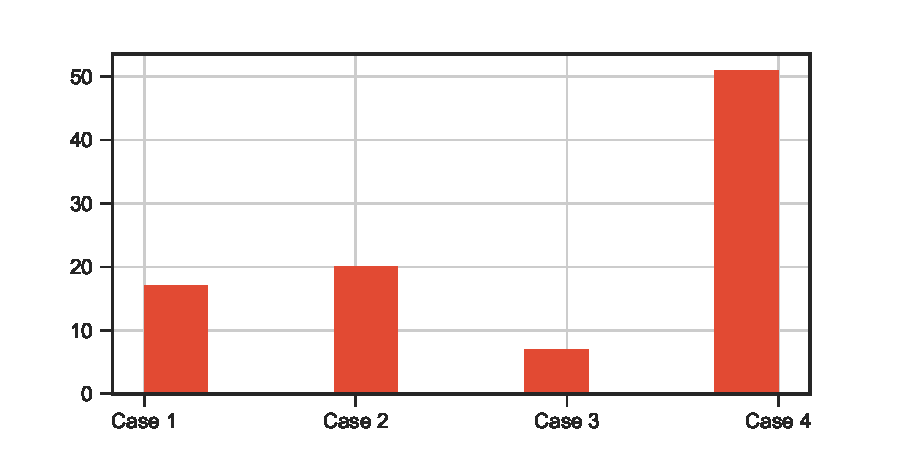
\includegraphics[width=0.45\textwidth]{figures/dataset_cases}
\caption{Preliminary results of current methods evaluated on Statement Granularity.}
\label{fig:dataset-cases}
\end{figure}


% It is important to mention, however, the most viewed questions are not representative of the entire \stackoverflow forum, but provide high quality answers and are (intuitively) the most suitable answers to 

\textbf{Methodology.} We manually analyze the answers to the most viewed Pandas question in \stackoverflow in the following manner:
\begin{enumerate}
	\item We only consider objective questions that have a source-code as the answer. Questions such as \diego{"Add here an example"} were not considered in this analysis. From the initial set, 10 questions were filtered out. 
	\item For each question, we analyze the \textit{accepted answer} and the \textit{most voted answer}, as in some cases, the accepted answer is not the most voted by the community. 5 questions have different most voted/accepted answers, hence we have a total of 95 answers to analyze.
    \item We extract the code snippet and filter out any non-parseable Python code. This step is done to remove comments, special characters from terminal code eg. \texttt{In} and \texttt{Out}, and any code output.
    \item We extract the solution by marking the lines we as developers would copy to use the solution in our own code. \diego{We need a crisp definition here...}
    \item We then classify each answer into one of the four categories presented.
\end{enumerate}

\textbf{Results. }
We present the analysis of the top 100 most viewed in \Cref{fig:pandas-top100-analysis}. 
\begin{itemize}
	\item Multiple Alternative Solutions (case 4) is the most prominent case with $\approx{54\%}$ of the answers. The most viewed questions often have well described answers with multiple alternatives. This shows the importance of an approach that can identify such cases.
    \item Single-line solution in Multi-line snippet was the second most common case with $\approx{21\%}$ of the analyzed answers.
    \item Trivial cases (Single-line snippet) appeared in third with $\approx{17\%}$ of the answers
    \item Multi-line appear only on $\approx{8\%}$ of the answers. 
\end{itemize}


% \begin{lstlisting}[caption={Setup embedded in the solution code (10715965).}, captionpos = b]
% # Question: Filter dataframe rows if value in column is in a set list of values

% df = pd.DataFrame(columns=['lib', 'qty1', 'qty2'])
% for i in range(5):
% 	df.loc[i] = [randint(-1,1) for n in range(3)]
% \end{lstlisting}

% \begin{lstlisting}[caption={Multiple alternatives solution in the snippet (11346283).}, captionpos = b]
% # Question: Renaming columns in pandas

% # Alternative 1
% df = df.rename(columns={'oldName1': 'newName1', 'oldName2': 'newName2'})
% # Alternative 2 
% df.rename(columns={'oldName1': 'newName1', 'oldName2': 'newName2'}, inplace=True)
% \end{lstlisting}








\subsection{Structuring Code}
Given that we have identified the solution code of a \stackoverflow question, we need to normalize the code and structure in a form that can be further reused semi-automatically \diego{maybe automatically?}.

\begin{itemize}
	\item Context dependent. Similarly to the Extracting Code problem to be able to normalize 
    \item Approach the problem in a API-centric way
    \begin{itemize}	
    	\item Identify the API calls as an entry-point.
        \item Use the API documentation to extract and normalize variable names.
    \end{itemize}
\end{itemize}








	
	\section{Approach}
	\subsection{Building the Dataset}

	\newcommand{\topquestions}{127}

\textbf{Crafting the Dataset.}
In order to evaluate our methods we have created a dataset containing manually extracted solutions from the SO questions.  

\begin{enumerate}
	\item We select the \topquestions most frequently viewed questions on SO tagged with \textit{pandas}. \diego{Add the new libraries}
    \item For each question we select the accepted and most voted answer to include in the dataset. In some cases, the accepted answer is not the most voted answer by the community.
    \item We manually extract the solution by \diego{We need a crisp methodology here}. The second author performed the extraction and each solution was also verified by the first author.  

\end{enumerate}




% To build the ground truth for the evaluation, we tag the most frequently viewed posts with tag \textit{pandas} have been tagged. We have manually identified solutions lines from the accepted answer posts as well as most voted answers. We are storing following details of a stackoverflow query in our tagged dataset.
       
%  \begin{center}
%  \begin{tabular}{ |c|c|c|c|c|c|c| } 
%  \hline
%        ques\_id & ques\_text & obj\_ques & ans\_id & sol\_id & solution & remarks \\
% \hline
% \end{tabular}
% \end{center}
% \textbf{ques\_id:} Question id is the the psot id of question, which will help extract details about the question from stack overflow\\
% \textbf{ques\_text:} Stack overflow question text\\
% \textbf{obj\_ques:} We are only considering objective questions textit{How-to} type questions. We are ignoring the subjective questions.\\
% \textbf{ans\_id:} Post id which is most voted as well as accepted answer (if they differ) for that question.\\
% \textbf{sol\_id:} There could be multiple solutions for a question in the same answer post. These different solutions are being assigned different solution ids.\\
% \textbf{solution:} Solution code (single line as well as multi line)\\
% \textbf{remarks:} Optional field for any remarks\\

\textbf{Example:}

\subsubsection{Building API Documentation base}
We have processed pandas api documentation\footnote{\url{https://pandas.pydata.org/pandas-docs/stable/api.html}} and stored the fully qualified method name and its description.

\subsection{Extracting API Documentation}

	
\textbf{Pandas.} We have processed pandas api documentation\footnote{\url{https://pandas.pydata.org/pandas-docs/stable/api.html}} and stored the fully qualified method name and its description.

\subsection{Methods and Heuristics}

	\diego{This section will be rewritten.}

\textbf{Heuristic H1: Look for the target API calls in Code Fragment}\\

After analyzing the stack overflow answers, it has been identified that, usually solutions are provided in terms of API method calls.\\
\textit{Hypothesis:} If there is API call in any statement, it as solution.\\
\textit{Approach:} Check the candidate code fragment for the presence of calls, method or attribute. In a code there could be zero or more methods (Calls). We have using AST parser to get all the methods present. This method labels the fragment as solution if at least one of the method is call to the API. If there is no method exists or no method is an API call, that fragment is rejected.\\

\textbf{Heuristic H2: Look for Non-constructors in Code Fragment}\\

While programming, usually first the objects are constructed and then methods are being called on them. While providing answers to a query, usually users first define the object and then write the actual solution code on these objects.\\
\textit{Hypothesis:} Any statement which only consists the constructor calls, could not be the solution.\\
\textit{Approach:} In API, the methods which are used to create objects, called constructors, has been annotated in API doc. All other methods/attributes are being called non-constructor here. We are using AST parser to get all the calls. If there is at least one non-constructor present in the statement, that statement is marked as solution.\\

\textbf{Heuristic H1H2: Non-constructors from API only}\\

In H1, statements having methods/attributes present in the API are identified as solution. In H2, all statements having non constructor calls are the solutions. These non-constructor call could be any thing. In this heuristic, scope of non-constructor call is defined as API specific calls. \\
\textit{Hypothesis:} Any statement which consists API specific non-constructor calls , is the solution.\\
\textit{Approach:} We first apply H1 to identify the API specific calls and then H2 to filter out constructor calls.\\


\textbf{Method M1: Look for API calls and Similarity between Stack overflow Question Text with the API Description}\\

In H1, we are just considering all the API calls to be as solution. There could be the case that an API call is the not the intended solution for that question. To avoid this shortcoming, we came up with the method M1 which considers the context of the post to get the relevance between API call and the question. This method utilizes similarity between question text and API description to get relevance among them.\\
We also identified that sometimes API description are too vague as below:

\textit{Method name}: pandas.rename\\
\textit{API description}: Alter axis label\\
\textit{Stack overflow question description}:Renaming columns in pandas\\\\
To overcome this kind of scenario, we enriched the API description with the fully qualified method name.

\textit{New API Description}: pandas rename Alter axis label

In this way, we will have two texts:
\begin{itemize}
	\item Question text for the post under consideration, say \textit{Text1}
	\item Fully Qualified Name of the method under consideration and its API description, say \textit{Text2}
\end{itemize}

We are using scikit-learn api\footnote{\url{http://scikit-learn.org/}} to generate TF-IDF vectors from these text and then using cosine similarity score as similarity measure. Cosine score 0 corresponds to \texttt{No Similarity} and 1 as \texttt{Total Similarity}.
	
\subsection{Cleaning parallel corpus for Machine Translation}

    \neelesh{This section is written by Neelesh}\\
This work \cite{Rahman:2019_CleaningStackOverflowforMT} proposed some cleaning approaches for text and code. We are hoping that our methods for extracting reusable code snippets will further reduce noisy code elements, improving the quality of parallel corpus. We will use these approaches as baseline for our work. Here is the summary of their approach.
\begin{itemize}
    \item \textbf{Extracting code elements} Extracted code elements using publicly available ACE tool \cite{Rigby:2013_DiscoveringEC} which was built for extracting code elements from free form StackOverlow text.
    \item \textbf{Text extraction and cleaning}
\begin{itemize}
    \item \textbf{C0: Raw data}: Raw post body text without any preprocessing. 
    \item \textbf{C1: Thread Title}: English corpus from thread title. Remove stop words and stem the text. Extract code from accepted answer.
    \item \textbf{C2: Standard NLP}: Keyword extraction, stopword removal and stemming of the text from post body.
    \item \textbf{C3: Raw data}: Extracting development tasks using TaskNavigator \cite{Treude:2015_TaskNav} from body text, stopword removal and stemming.
\end{itemize}
\end{itemize}

Unfortunately ACE tool is built for Java which was not suitable for our study of pandas library which is used by python programmers. We looked into the corpus\footnote{\url{https://github.com/mrsumitbd/SOParallelCorpusReplication}} shared by \cite{Rahman:2019_CleaningStackOverflowforMT} and found that ACE extracts method calls. Our method of cleaning code snippet also produces method calls. We used these extracted code elements for our study. This way we are also using method calls and since same code elements will be used for all the approaches so our study is not affected by any of the method/call extraction approach.\\\\
We adapted the best two approaches \textbf{C1: Thread Title} and \textbf{C2: Standard NLP} for extracting and cleaning text. We further cleaned the code elements using our approaches for finding reusable code snippets to filter out noisy code elements.
\begin{itemize}
    \item \textbf{All}: All the code elements. This will serve as baseline.
    \item \textbf{H1}: Filter noisy code elements using H1.
    \item \textbf{H1H2}: Filter noisy code elements using H1H2.
    \item \textbf{M1}: Filter noisy code elements using H1H2.
\end{itemize}



	
	\section{Evaluation}
	\subsection{Preprocessing SO Code Snippet.}

We are using Stackoverflow dump as our dataset. Cleaning of the stack overflow posts is needed to get clean code from it where each line should valid parsable code.
\begin{enumerate}        
	\item The code are present inside \texttt{<pre><code>} tag. We extracted all the code snippet present inside this tag for all the post.    
	\item Remove special characters from beginning of the line: There are post where the code was written starting with special characters like the following \texttt{>>> df.read\_csv(f)}. Except few special characters, python lines should not start with any special character. In this preprocessing step we removed any such special characters
          
	\item Removing Ipython terminal like codes: Several code fragments have the IPython tokens, IN and OUT, which has been removed. We only pick the code fragment between IN and OUT.
    \begin{lstlisting}
In [4]: df.groupby('A').sum()
Out[4]:
	1 5
	4 6
\end{lstlisting}
    
    \item Validating through Python AST: Finally the lines are passed through the python ast module to check for validity of the code.
    
\end{enumerate}

We have processed posts of stack overflow dump to clean the code in our preprocessing step.

\subsection{Evaluation Methods for Reusable Code Snippet}
     
To evaluate our approach we compare the code yielded by each method against our tagged dataset using two methods: Full solution comparison and statement granularity comparison.



\textbf{Full solution granularity.}
Compare the entire solution extracted by our approach against the manually crafted dataset.
\begin{itemize} 
	\item This is the most important evaluation to argument the usefulness of our methods.  
    \item We are only interested on precision, that is, a solution provided must be correct.
    \item However, we might weight differently incomplete solutions and suboptimal solution (solution with unessential statements).
\end{itemize}

\textbf{Statement granularity.}
Compare the each statement extracted by our methods against the statements of the solution.
\begin{itemize} 
	\item This evaluation allow us to better measure the extracted solution code in terms of accuracy, F1, precision and recall
    \item Recall is the most important aspect here, however recall is very sensitive to our high quality dataset as top questions often have short responses. 
    \item We have to think whether it does measure properly our main concern here: extraction of correct code template from Stack Overflow.
\end{itemize}

\subsection{Evaluation Methods for Cleaning Parallel Corpus for Machine Translation}
\neelesh{This section is written by Neelesh}\\
As reported in \cite{Rahman:2019_CleaningStackOverflowforMT} one of the limitations of MT is that there is no straightforward mechanism to evaluate quality of corpus except the actual training which takes a considerable amount of time. We used evaluation method \textit{Per-Word Alignment Entropy} proposed by the same work. They create simple maximum-likelihood machine translation models. Each English word is aligned to one of more code elements based on maximum-likelihood. The lower the alignment entropy for each English word the stronger the mapping to specific code elements and better the model.




% Our tagged dataset contains the solution code for the answer post. This tagged dataset will serve the purpose of ground truth. The stack overflow dump will be used for testing against this ground truth.

% The codes could be single line or multi-line. Right now, we are considering the \textit{Single line codes} for our evaluation.
% To evaluate we do the following steps:
% \begin{enumerate}
%   \item Iteratively pick answer posts from processed stack overflow dump and look for its presence in our tagged data set using the post ids.
%   \item If the post under consideration is present in the dataset Iterate through lines of code.
%   \item Our methods process takes one line at a time and predicts whether to label it as a solution or not.
%   \item This candidate line is then checked into the tagged dataset solution list and if it is present we mark it as actual solution. We use full text matching to check the presence of a line in solution set.\\
% \end{enumerate}

% For each line of each post of stack overflow dump, we calculate TP, TN, FP and FN as follows:\\\\
% \textbf{TP True Positive:} Method predicts the line as \textit{solution} and the line is also \textit{present} in solution list\\
% \textbf{TN True Negative:} Method predicts the line as \textit{not solution} and the line is \textit{not present} in solution list.\\
% \textbf{FP False Positive:} Method predicts the line as \textit{solution} and the line is \textit{not present} in solution list.\\
% \textbf{FN False Negative:} Method predicts the line as \textit{not solution} and the line is \textit{present} in solution list.\\\\
% We are using metrics Accuracy, Precision, Recall and F1 as define below:\\\\
% \[ Accuracy: \frac{TP+TN}{TP+TN+FP+FN} \]
% \[Precision: \frac{TP}{TP+FP} \]
% \[Recall: \frac{TP}{TP+FN} \]
% \[F1: \frac{2*Precision*Recall}{Precision+Recall} \]


	
	\section{Results}
	Results goes here...

\subsection{Preliminary Results on finding solution snippet}
In our preliminary results we have found the following:

\subsection{Results on cleaning SO for machine translation}
\neelesh{This section is written by Neelesh}\\
We plot the per word alignment distribution as 5 point summary via box plot in \ref{fig:preliminary-results-c1} and \ref{fig:preliminary-results-c2}. The box shows the IQR which covers the 50\% of the values. The horizontal line in the box is the median. Lower the median entropy and IQR width, better the model. Although each English word maps to the limited set of code elements, there are outlier English words that map to a large number of possible elements (shown as black circles). From the table \ref{tab:alignment-entropy-mt} it can be deduced that our approaches further reduce the entropy compared to baseline.

\begin{table}[b]
\label{tab:alignment-entropy-mt}
\caption{Median Alignment Entropy}
\begin{tabular}{1 1 1 1 1}
		 \textbf{Approaches} 		& \textbf{All-Baseline} 		& \textbf{H1} 		& \textbf{H1H2} 	& \textbf{M1}
		 \\ 
		 \hline
		 	C1 (Title Only)						& 0.258					& 0.007				& 				& 2.59e-09
		 	\\
		 	\hline
		 	C2 (Standard NLP)						& 0.010				& 0.0002				& 0.0002				& 1.78e-09
		 	\\ 
		 \hline

\end{tabular}
\end{table}


\begin{figure}[!t]
\centering
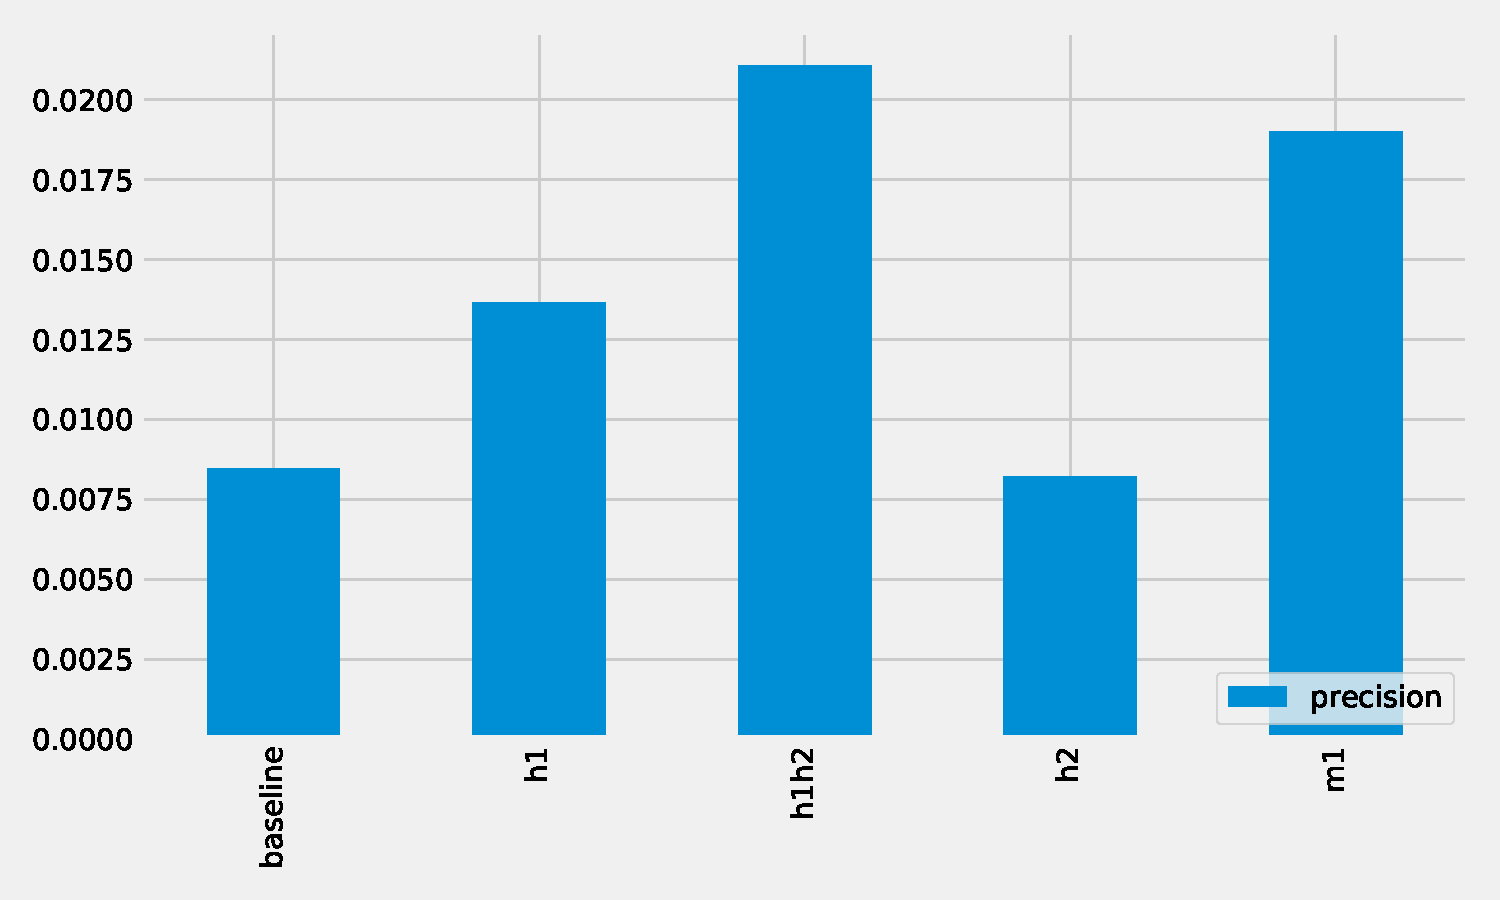
\includegraphics[width=2.5in]{figures/all-methods-block}
\caption{Preliminary results of current methods evaluated on Full Solution method. \diego{Note the y-axis scale.} }
\label{fig:preliminary-results-block}
\end{figure}


\begin{figure}[!t]
\centering
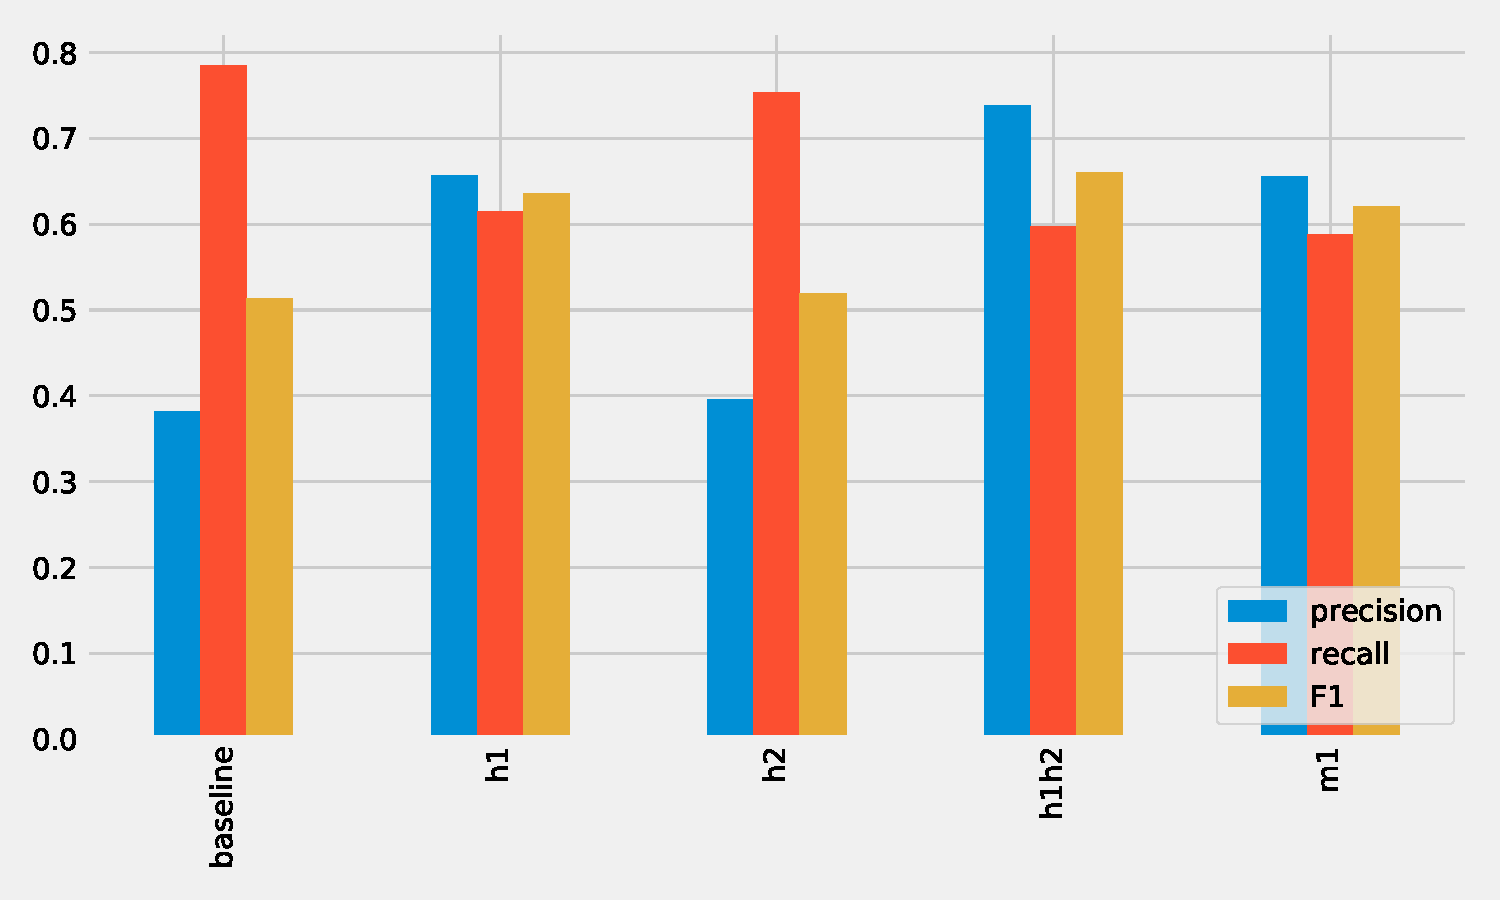
\includegraphics[width=2.5in]{figures/all-methods-line.pdf}
\caption{Preliminary results of current methods evaluated on Statement Granularity.}
\label{fig:preliminary-results-line}
\end{figure}


\begin{figure}[!t]
\centering
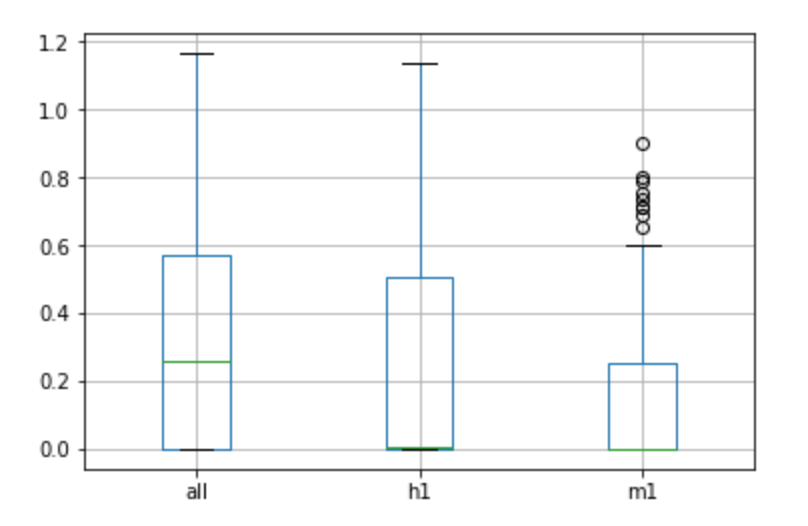
\includegraphics[width=2.5in]{figures/title-machine-translation.png}
\caption{Distribution of per-word alignment maximum likelihood alignment entropy. The more left skewed a distribution, lower the entropy, and the higher is predictive power. C1-Thread Title approach of Cleaning SO for Machine Translation.}
\label{fig:preliminary-results-c1}
\end{figure}


\begin{figure}[!t]
\centering
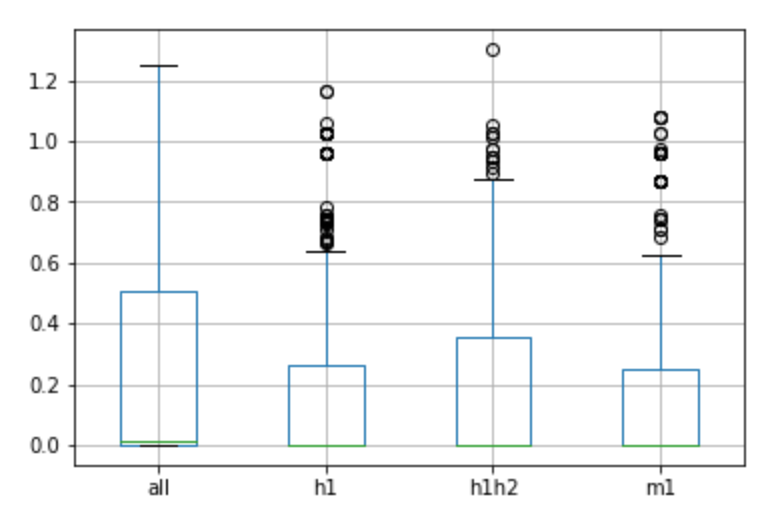
\includegraphics[width=2.5in]{figures/post-body-machine-translation.png}
\caption{Distribution of per-word alignment maximum likelihood alignment entropy. The more left skewed a distribution, lower the entropy, and the higher is predictive power. C2-Standard NLP approach of Cleaning SO for Machine Translation.}
\label{fig:preliminary-results-c2}
\end{figure}
	
	\section{Related Work}
	% Blank page just to separate Related work at the moment
\newpage
\phantom{blabla}
\newpage

Various studies have investigated the use of SO code on software engineering.


\subsection{Empirical Studies on SO}

% Form query to Usable Code
Yang \cite{Yang:2016_FromQueryToUsableCode} assessed the usability of code snippets.
\begin{itemize}
	\item Usability of code inferred by compiling and running the source-code
	\item Python and JavaScript proved to be the languages with highest rate of usable code
\end{itemize}

% Stack Overflow on GitHub: Any Snippets There?
In \cite{Yang:2017_AnySnippetsThere} authors have investigated the occurrence of SO code in Github projects.
\begin{itemize}
	\item Analyze 909k Python projects containing 290M function definitions from \github.
	\item Analyze 1.9M Python snippets from Stack Overflow
	\item Quantitative analysis: exact duplication between SO and \github exists but is rare, much less than 1\%. Although the percentage is not very large the numbers are in thousands.
	\item Qualitative analysis: Vast majority of duplicated codes are very small.
	\item \diego{We have to further investigate the issues found in this paper. If the percentage of usage is so small, we might run into trouble to find enough data in \github projects.}
\end{itemize}

% Stack Overflow: A code laundering platform?
An \textit{et al.} \cite{An:2017_SOACodeLaunderingPlatform} investigated the unethical reuse of Stack Overflow code in real projects.
\begin{itemize}
	\item Study made on 339 Android applications
	\item Vast majority \diego{(add number here later)} of code snippets used in projects do not report the license from SO (potential code violation).
\end{itemize}

Baltes \textit{et al.}~\cite{Baltes:2017_AttributionRequired} also investigates the occurrences of copied SO snippets in GitHub projects.
\begin{itemize}
	\item Only 23\% of the identified clones of Java snippets have link that attributes it to the original SO post.
    \item 
\end{itemize}

% 
Gabel \textit{et al.} \cite{Gabel:2010_UniquenessOfCode} investigated the property of uniqueness of code in software projects.
\begin{itemize}
	\item General lack of uniqueness in software in levels of granularity equivalent to approximately one to seven lines of code.
	\item Pervasive phenomenon: it happens across projects ans programming languages.
\end{itemize}


\textbf{Dataset.} Ponzanelli \textit{et al.} provided a structured dataset for SO \cite{Ponzanelli:2015:STORM_SODataset} for Java programs.
\begin{itemize}
	\item Model each code as a heterogeneous abstract syntax tree \diego{check this in details}.
	\item Link available at \footnote{https://stormed.inf.usi.ch/}.
	\item \diego{We need to check this dataset if we want to add as a contribution our own manually tuned dataset.}
\end{itemize}

\subsection{Using SO in Software Engineering}

\textbf{Code Recommender.} Ponzanelli's group has worked on several approaches that harness Stack Overflow code snippets into code recommender. 

In \cite{Ponzanelli:2014_MiningSOTurnIDE,Ponzanelli:2014_Prompter}, the authors presented the core idea of mining Stack Overflow to provide Prompter, a IDE plugin that:
\begin{itemize}
	\item Continuously monitor developer's code and try to find the best "next" code, based on SO usage.
    \item Code is ranked based on the similarity of currents developer code (clone code detection).
    \item \diego{Check if authors only mine SO or also GitHub}
\end{itemize}

SeaHawk~\cite{Ponzanelli:2013_SeaHawk} (from the same group) integrates Stack Overflow search with an Eclipse IDE plugin.
\begin{itemize}
	\item Formulates queries automatically from the active context of the IDE
    \item Ranked and interactive list of results
    \item Lets user import code 
    \item YouTube video~\footnote{https://www.youtube.com/watch?v=DkqhiU9FYPI}
    \item \diego{There is no transformation of the code involved (no automated transplantation).}
\end{itemize}

In a recent study~\cite{Ponzanelli:2017_Holistic} addresses the problem of heterogeneity of Stack Overflow posts. In this work the authors propose Libra
\begin{itemize}
	\item Integrate IDE with the Google search in the Web Browser
    \item Classify the posts based on the relevance to the developer's context
    \item Project page \footnote{http://libra.inf.usi.ch/}
	\item YouTube video \footnote{https://www.youtube.com/watch?v=yb69hYwTYyA}
    \item \diego{Our contribution is orthogonal to the contributions proposed by Ponzanelli's group.}
\end{itemize}

\textbf{Program Repair.} In "Mining Stack Overflow for Program Repair"~\footnote{www.cs.sjtu.edu.cn/~zhonghao/paper/minstackoverflow.pdf} (to be published in SANER`18), the authors mined the SO to provide templates for automated program repair:
\begin{itemize}
	\item Template patches are generated based on the Question-Answer code. 
    \item 13 templates were mined from SO
    \item Templates used on Defects4J to fix 23 bugs
\end{itemize}

In~\cite{Nielebock:2017_TowardsAPIAutomaticProgramRepair}, authors introduce the concept of API-Specific Automatic Program Repair. 
\begin{itemize}
	\item \diego{Short paper on ASE 2017}
    \item Discusses the concept of having API-specific repair patches
    \item Points at the challenge of "Extracting API-specific information", which we are tackling. \diego{This can be further used for motivation}.
\end{itemize}


	
	\section{Conclusion}
	Discussion goes here...
	
	
	%%
	%% The acknowledgments section is defined using the "acks" environment
	%% (and NOT an unnumbered section). This ensures the proper
	%% identification of the section in the article metadata, and the
	%% consistent spelling of the heading.
	\begin{acks}
		%To Robert, for the bagels and explaining CMYK and color spaces.
	\end{acks}
	
	%%
	%% The next two lines define the bibliography style to be used, and
	%% the bibliography file.
	\bibliographystyle{ACM-Reference-Format}
	\bibliography{bibliography}
	
	%%
	%% If your work has an appendix, this is the place to put it.
	\appendix
	
\end{document}
\endinput
%%
%% End of file `sample-sigconf.tex'.



